
沒有必要全部想寫的都寫上去

\chapter{\textcolor{yellow}{analysis 先}}
\chapter{\textcolor{red}{waveform 先!}}

\section{\textcolor{lime}{最小作用量:Ch4 就照跑就好,其他都別管;}}
\section{\textcolor{lime}{理論上老師要的額外分析加上這些就夠細緻了}}
% 然後就 Ch5、摘要中英、題目

例如 phone group 的有緣再寫,
alignment, triphone, speaker 有空再寫
70\% 有緣再說
CPCfix, framefix 有空再說

\centering

------------------------

你想,你 707 之後也沒有電腦了,所以也沒有什麼之後再來跑實驗的餘裕。你就想之後就不要研究了,啊現在想 demo 的也就只有現在可以做。之後放棄掉那些本質有的沒的,聽命辦事就行。

想想:要嗎過高求太好做不到,要嗎過低連有都不能有欺騙自己
真正的先求有再求好的那個「求有」其實是非常艱辛的,至少對我如此。\textcolor{yellow}{(對別人可能是輕而易舉。所以說為什麼我很爛,但沒人在乎你很爛,很爛就該閉嘴滾一邊去。現在就是演戲裝厲害而已畢竟我就是很爛)}

==============

標註
碼字(Codeword)
pattern 類型


% ~~~~~~~~~~~~~~~~~~~~~~~~~~
% ~~~~~~~~~~~~~~~~~~~~~~~~~~
% ~~~~~~~~~~~~~~~~~~~~~~~~~~

% ref: https://tex.stackexchange.com/questions/24496/use-caption-and-long-description-for-figure
\begin{figure}
    \centering
    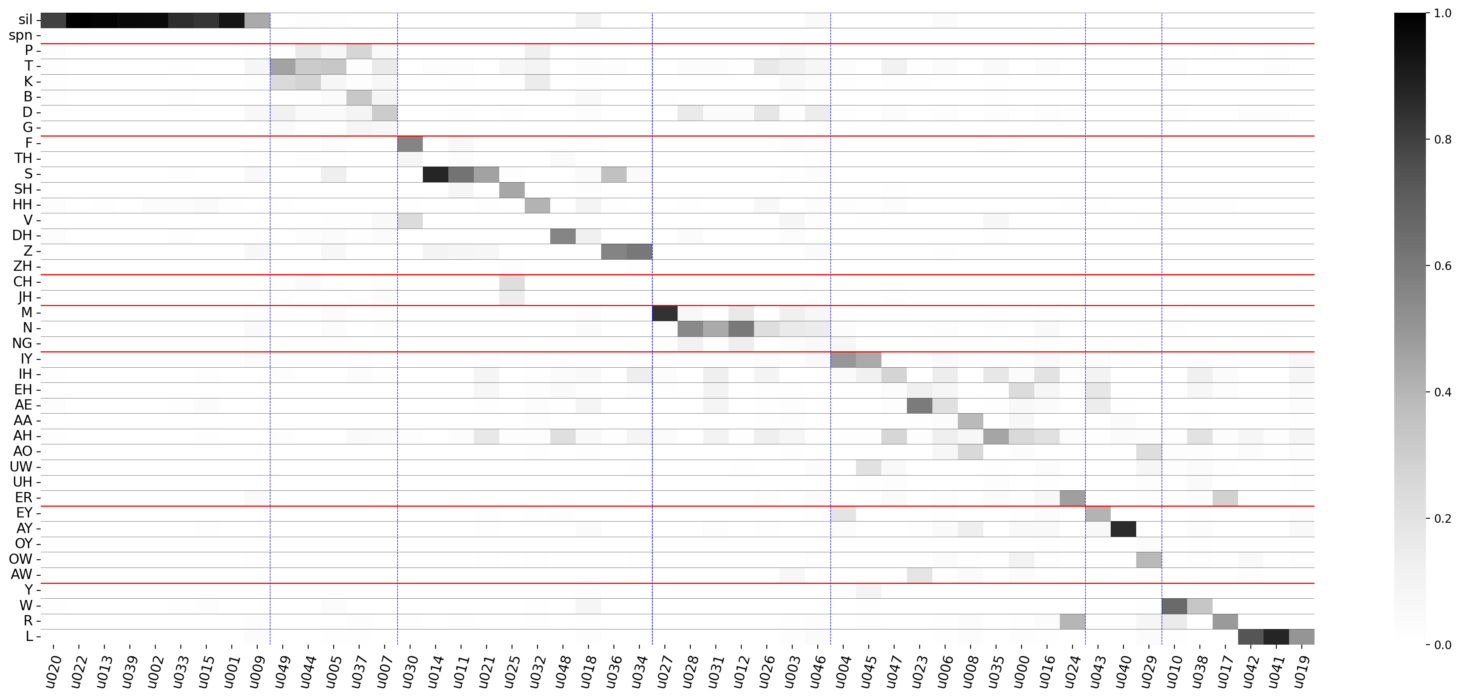
\includegraphics[width=1\linewidth]{figures/hubert-50-givenunit-byphn.png}
    \caption[]{
        HuBERT 模型、分群數為 50 之離散單元
        }  % \medskip % \small
                       與音位標註的條件機率,依照語音學分類排序的分佈圖
    \label{fig:hubert-50-givenunit-byphn}
\end{figure}
